\section{Experimental protocol}
\label{sec:protocol}

\subsection{Corpora, checkpoints, and evaluation units}
The principal assessment contains 11,306 VLR clips, 1,243 LRS2 clips, 934
Spanish clips, and 1,167 ViCocktail clips. VLR and ViCocktail provide two
Vietnamese corpus/model conditions; LRS2 provides English; the Spanish
evaluation uses the MuAViC/mTEDx material
\citep{vlr2026dataset,afouras2022deep,anwar2023muavic,nguyen2025vicocktail}.
The comparison is paired within each corpus and is not pooled across languages.
Recording-source counts are 61, 354, 12, and 20, respectively.
These identifiers group clips from the same source and are not verified
speaker identities.
The prepared clips also differ in duration: means are 5.78 s for VLR, 1.64 s
for LRS2, 5.91 s for Spanish and 5.83 s for ViCocktail. Appendix~\ref{app:corpus}
reports the distributions, actual context availability and recording-source
weights for these exact assessment cohorts.

\begin{figure}[tb]
 \centering
 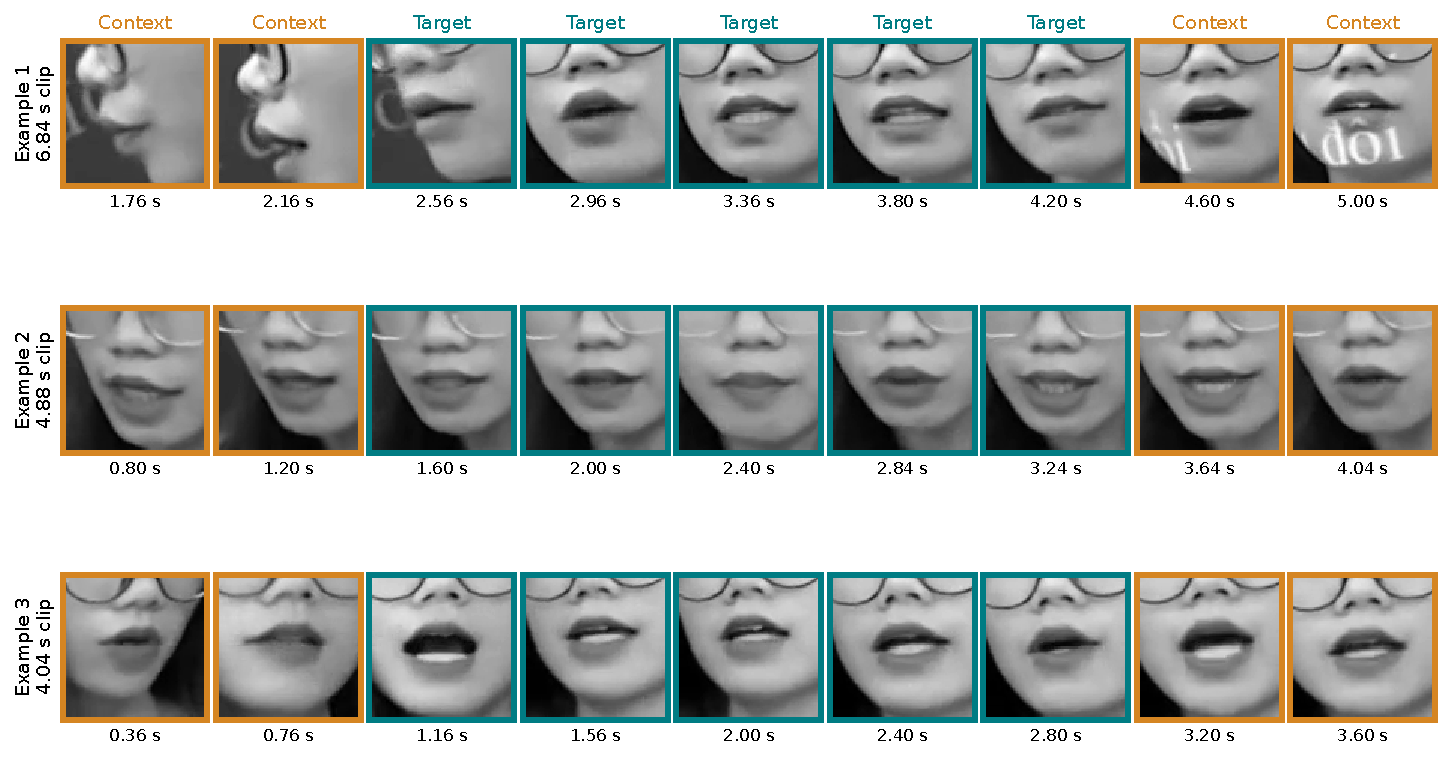
\includegraphics[width=\linewidth]{fig_Dataset_Examples.pdf}
 \caption{Actual prepared VLR mouth-region inputs for three centered requests.
 Each row shows nine sampled frames from an observed interval with a two-second
 target (teal borders) and up to 0.64 seconds of context on each side (orange).
 Times are relative to the original clip. The inputs retain their original
 resolution, motion blur and overlays; they are neither retouched nor generated.
 Examples were selected by clip identifier without using recognition outcomes;
 distinct recording IDs do not imply distinct speakers. Images adapted from
 VLR v2 \citep{vlr2026dataset}, CC BY 4.0.}
 \label{fig:dataset-examples}
\end{figure}

\begin{figure}[tb]
 \centering
 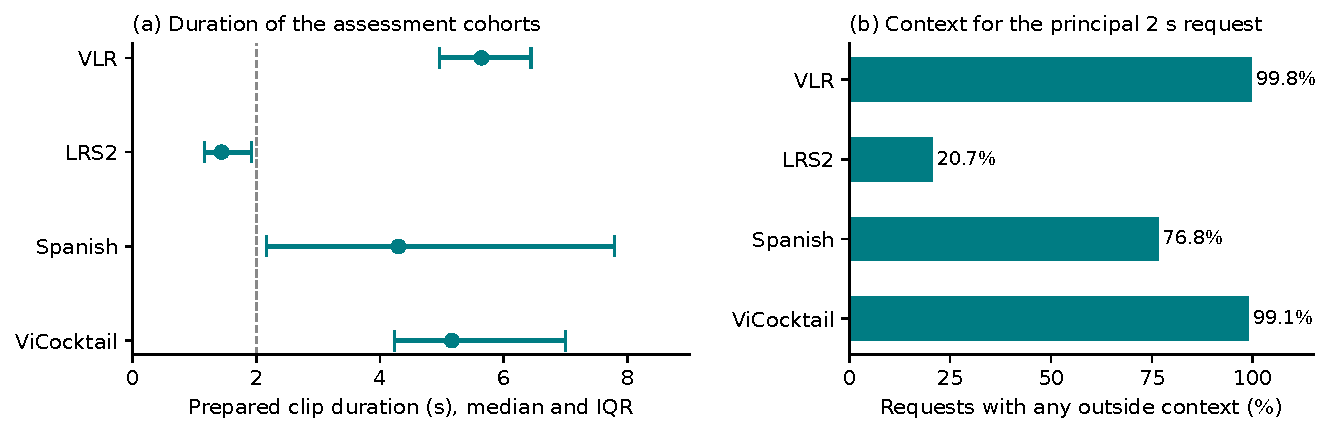
\includegraphics[width=\linewidth]{fig_Corpus_Geometry.pdf}
 \caption{Geometry of the exact four assessment cohorts. (a) Median clip duration
 with interquartile range; the dashed line marks the nominal two-second target.
 (b) Fraction of principal requests with any real video outside their target.
 These are cohort descriptions, not whole-dataset or language-population
 estimates. The short LRS2 clips provide less opportunity to admit context.}
 \label{fig:corpus-geometry}
\end{figure}
Figure~\ref{fig:dataset-examples} illustrates the visual input and the distinction
between target and context. Figure~\ref{fig:corpus-geometry} relates that distinction
to the evaluated clip durations. A context allowance specifies a maximum;
the actual neighboring evidence depends on clip length and request position.

Each setting uses a frozen, language-compatible checkpoint and its native
tokenizer. English uses the published Auto-AVSR visual model trained with
LRS2/LRS3/VoxCeleb2/AVSpeech material \citep{ma2023autoavsr}.
VLR uses our previously adapted T0 checkpoint (seed 17, selected at step 3,000),
and ViCocktail uses our separately trained Vietnamese Auto-AVSR checkpoint
(epoch 13). These are local model instances, not checkpoints released by
the respective dataset authors.
Spanish uses the released \texttt{vsr-low} model of \citet{yeo2024vsrlow},
trained with mTEDx, VoxCeleb2, and AVSpeech material. Its release filename is
\path{es_mted_vox_avs_wer_45.7.pth}; the English release is
\path{vsr_trlrs2lrs3vox2avsp_base.pth}.
The output vocabularies contain 2,002 classes for the two Vietnamese models,
5,049 for English, and 1,006 for Spanish, with the corresponding tokenizer
and special-token conventions retained.
The inference procedure reuses these checkpoints without additional training.

Decoder calibration and assessment are clip- and source-disjoint within the
present protocol. Calibration sizes are 512 for VLR, English, and ViCocktail,
and 286 for Spanish. Assessment membership is frozen before these comparisons.
The material was available during earlier research, so this is an expanded
controlled evaluation rather than a newly collected independent replication.
Eligibility requires usable video and word timing; one VLR clip and 78 of
1,012 Spanish candidate clips are timing-ineligible. No clip is removed because
of its recognition error.

Calibration compares greedy CTC, pure CTC beam search, and hybrid decoding
with CTC weights 0.1, 0.5, and 0.9. Beam searches use width 40 and the
hybrid length bonus is zero. VLR selects greedy decoding for A/B/C and
hybrid weight 0.5 for F. The other three settings select hybrid weight 0.1
for A/C/F and 0.5 for B. Uniform allocation inherits C's prediction and
decoder. These choices are retained throughout the assessment and duration
experiments; matched-decoder comparisons remove this between-arm choice.

We report corpus-level edit error
\begin{equation}
 \mathrm{WER}=100\,\frac{\sum_i(S_i+D_i+I_i)}{\sum_i N_i},
\end{equation}
where the counts refer to the same requested reference text for all compared
arms. Unicode NFC normalization, lowercasing, and whitespace normalization are
fixed. Vietnamese uses whitespace-delimited orthographic units, which need not
coincide with linguistic words. Absolute error rates therefore do not support
a cross-language difficulty ranking.

\subsection{Target construction and reference timing}
The principal setting uses a target of at most 50 frames at 25 fps and up to
16 context frames on either side. Start, center, and end placements are assigned
deterministically from clip identifiers. Clips shorter than the target are
retained as whole-clip targets, rather than excluded to favor context methods.
Within an experimental cell, all arms have the same target reference.

Word midpoints from the fixed reference timing determine target membership.
Whole-clip targets retain the complete original transcript. The reference
transcript and its timing are accessed only for scoring; inference uses video,
predicted tokens, and predicted alignment. VLR retains the supplied
ASR-derived transcript and word spans. LRS2 and Spanish use audio-CTC
forced alignment of their corpus transcripts; ViCocktail uses its native
test labels, reported as manually transcribed by the dataset authors,
with audio-CTC word alignment. Audio is used only to prepare evaluation
references, never by the visual recognizer or prediction-alignment procedure.
These automatic word times are not independent human boundary annotations.
Reference-clock perturbations of \(\pm40,\pm80,\pm160\) ms and an overlap-based
ownership convention examine sensitivity to this evaluation choice.

\subsection{Controlled experiments}
The duration experiment varies nominal target length over 1, 2, and 3 seconds
and maximum context per side over 0, 0.32, and 0.64 seconds. It includes 1,024
clips each for VLR, LRS2, and ViCocktail, and all 934 eligible Spanish clips.
The decoder choices remain those calibrated at the principal operating point;
each duration cell is evaluated without selecting a new decoder.
Within each target
length, it compares the same clips and requested text. Changing target length
changes the reference content, so the smallest raw WER across lengths is not
interpreted as an optimal segmentation duration.

Context interventions use 256 clips per corpus. They compare real context
with equal-length repeated-boundary padding, reversed margins, and left-only
or right-only context while preserving target pixels. The primary padding
contrast uses clips that actually have outside context.
The full-transcript experiment uses 512 clips per corpus. For nominal target
budget \(L\), a clip of \(T\) frames is partitioned into
\(K=\lceil T/L\rceil\) balanced, nonoverlapping target intervals. Direct and
projected sliding share that schedule and concatenate their outputs in time
order. A further control joins contextual target CTC scores before decoding
once, separating text concatenation from repeated local recognition.

For query costs, 32 duration-stratified calibration clips per corpus are
evaluated on a GTX 1650 Ti in float32, at batch size one with two CPU threads
and one GPU worker. One, three, and five
requested intervals are deduplicated when short clips yield identical queries.
Development-selected systems and a separate matched pure-CTC control use
the exact same clips and query schedules. In the matched control, every arm
uses beam width 40 and token-pruning limit 64 without decoder recalibration.
Three fresh sessions are run per scenario, with arm order rotated by clip
and repetition. We first take within-clip medians, then summarize their
median and 95th percentile across clips. Recognition and required allocation are timed
with the model resident; input loading is measured separately. The experiment
also measures repeat lookup from populated caches. It does not measure
raw-video face tracking, live acquisition delay, or human editing time.

\subsection{Uncertainty and comparison families}
The eight principal contrasts are projection versus crop-first and projection
versus contextual direct in each corpus. We use paired source-cluster
bootstrap resampling with 10,000 draws. Bonferroni adjustment gives
99.375\% individual percentile intervals for this family. The interval
construction was chosen at analysis time for the fixed comparison family;
it has approximate bootstrap coverage. Other intervals describe explanatory
contrasts at pointwise 95\% coverage. Limited source counts, especially in
Spanish, constrain the precision and generality of those comparisons.

An explanatory analysis recomputes matched greedy and pure-CTC intervals
from the frozen predictions and partitions each cohort by actual outside
context: none, left only, right only, or both. These post-hoc explanatory
comparisons use the same 10,000-draw paired-source procedure with pointwise
95\% intervals; they do not alter the primary comparison family or decoder
selection. Geometry is read from the recorded input and target coordinates.
